\documentclass[10pt]{article}

\usepackage{caption}
\usepackage{float}
\usepackage{courier}
\usepackage{xspace}
\usepackage{listings}
\usepackage{graphicx}
\usepackage{mdframed}

\lstset{%basicstyle=\ttfamily
  language=C,
  basicstyle=\ttfamily\footnotesize,
  frame=lrbt,
  morekeywords={action,apply,bit,bool,%
const,control,default,else,%
enum,error,extern,exit,%
false,header,header_union,if,%
in,inout,int,match_kind,%
package,parser,out,return,%
select,state,struct,switch,%
table,transition,true,tuple%
typedef,varbit,verify,void,%
%
abstract,interface,class,virtual% used for IR
}
}
\newcommand{\PFOUR}{P4\xspace}
\newcommand{\code}[1]{\texttt{#1}}
\newcommand{\keyword}[1]{{\bf \texttt{#1}}}
\newcommand{\vonemodel}{\code{v1model}\xspace}

\title{Linux network programming with \PFOUR}
\author{William Tu\\
  VMware Inc.\\
  \texttt{tuc@vmware.com}
  \and
  Fabian Ruffy\\
  University of British Columbia\\
  \texttt{fruffy@cs.ubc.ca}
  \and
  Mihai Budiu\\
  VMware Research\\
  \texttt{mbudiu@vmware.com}
}
\date{}

\begin{document}
\maketitle

\begin{abstract}
  \PFOUR is a programming language for implementing network dataplanes.
\end{abstract}

\section{Introduction}\label{sec:introduction}

\section{Background}\label{sec:bacground}

\subsection{P4}

(This section is adapted from~\cite{budiu-osr17}.)  P4 is a relatively
simple, statically-typed programming language, with a syntax based on
C, designed to express transformations of network packets.

The core abstractions provided by the P4 language are listed in
Figure~\ref{fig:abstractions}.  P4 provides no support for pointers,
dynamic memory allocation, floating-point numbers, or recursive
functions; looping constructs are only allowed within parsers.

\definecolor{grey}{rgb}{0.9, 0.9, 0.9}
\global\mdfdefinestyle{mdstyle}{%
innerleftmargin=.3cm,rightmargin=.3cm,backgroundcolor=grey}
\begin{figure*}[h]
  \begin{mdframed}[style=mdstyle]
    \begin{description}
\item[Headers] describe the format (the set of fields, their ordering
  and sizes) of each header within a network packet.
\item[User-defined metadata] are user-defined data structures
  associated with each packet.
\item[Intrinsic metadata] is information provided or consumed by the
  target, associated with each packet (e.g., the input port where a
  packet has been received, or the output port where a packet has to
  be forwarded).
\item[Parsers] describe the permitted header sequences within received
  packets, how to identify those header sequences, and the headers to
  extract from packets.  Parsers are expressed as state-machines.
\item[Actions] are code fragments that describe how packet header
  fields and metadata are manipulated. Actions may include parameters
  supplied by the control-plane at run time (actions are closures
  created by the control-plane and executed by the data-plane).
\item[Tables] associate user-defined keys with actions.  P4 tables
  generalize traditional switch tables; they can be used to implement
  routing tables, flow lookup tables, access-control lists, and other
  user-defined table types, including complex decisions depending on
  many fields.  At runtime tables behave as match-action
  units~\cite{bosshart-sigcomm13}, processing data in three steps:
  \begin{itemize}
    \item Construct lookup keys from packet fields or computed
      metadata,
    \item Perform lookup in a table populated by the control-plane,
      using the constructed key, and retrieving an action (including
      the associated parameters),
    \item Finally, execute the obtained action, which can modify the
      headers or metadata.
  \end{itemize}
\item[Control] blocks are imperative programs describing the
  data-dependent packet processing including the data-dependent
  sequence of table invocations.
\item[Deparsing] is the construction of outgoing packets from the
  computed headers.
\item[Extern objects] are library constructs that can be manipulated
  by a P4 program through well-defined APIs, but whose internal
  behavior is hardwired (e.g., checksum units) and hence not
  programmable using P4.
\item[Architecture definition:] a set of declarations that describes
  the programmable parts of a network processing device.
    \end{description}
  \end{mdframed}
  \caption{\sl Core abstractions of the P4 programming language.\label{fig:abstractions}}
\end{figure*}

\subsection{P4 Architectures}

P4 allows programs to execute on arbitrary \emph{targets}.  Targets
differ in their functionality, (e.g., a switch has to forward packets,
a network card has to receive or transmit packets, and a firewall has
to block or allow packets), and also in their custom capabilities
(e.g., ASICs may provide associative TCAM memories or custom checksum
computation hardware units, while an FPGA switch may allow users to
implement custom queueing disciplines).  P4 embraces this diversity of
targets and provides some language mechanisms to express it.

\begin{figure}[h]
  \centerline{\includegraphics[width=.5\textwidth,clip,trim=1in 0.9in
      .8in 1.8in]{architecture.pdf}}
  \caption{\sl Generic abstract packet-processing engine programmable
    in P4.  The blocks labeled with P4 are programmable in P4; the
    surrounding block is fixed-function
    logic.\label{fig:architecture}}
\end{figure}

Figure~\ref{fig:architecture} is an abstract view of how a P4 program
interacts with the data-plane of a packet-processing engine.  The
data-plane is a fixed-function device that provides several
programmable ``holes''.  The user writes a P4 program to specify the
behavior of each hole.  The target manufacturer describes the
interfaces between the programmable blocks and the surrounding
fixed-function blocks.  These interfaces are target-specific.  Note
that the fixed-function part can be software, hardware, firmware, or a
mixture.

A P4 architecture file is expected to contain declarations of types,
constants, and a description of the control and parser blocks that the
users need to implement.  Section~\ref{sec:ebpf} contains an example
P4 architecture description file.

\subsection{eBPF for network processing}

(This section is adapted from~\cite{p4-ebpf-backend}.)  eBPF is a
acronym that stands for Extended Berkeley Packet Filters. In essence
eBPF is a low-level programming language (similar to machine code);
eBPF programs are traditionally executed by a virtual machine that
resides in the Linux kernel. eBPF programs can be inserted and removed
from a live kernel using dynamic code instrumentation. The main
feature of eBPF programs is their static safety: prior to execution
all eBPF programs have to be validated as being safe, and unsafe
programs cannot be executed. A safe program provably cannot compromise
the machine it is running on:
\begin{itemize}
\item it can only access a restricted memory region (on the local
  stack),
\item it can run only for a limited amount of time; during execution
  it cannot block, sleep or take any locks,
\item it cannot use any kernel resources with the exception of a
  limited set of kernel services which have been specifically
  whitelisted, including operations to manipulate tables (described
  below)
\end{itemize}

\subsubsection{Kernel hooks}

eBPF programs are inserted into the kernel using hooks. There are
several types of hooks available:

\begin{itemize}
\item function entry points can act as hooks; attaching an eBPF
  program to a function foo() will cause the eBPF program to execute
  every time some kernel thread executes foo().

\item eBPF programs can also be attached using the Linux Traffic
  Control (TC) subsystem, in the network packet processing
  datapath. Such programs can be used as TC classifiers and actions.

\item eBPF programs can also be attached to sockets or network
  interfaces. In this case they can be used for processing packets
  that flow through the socket/interface.
\end{itemize}

\subsubsection{eBPF Maps}

The eBPF runtime exposes a bi-directional kernel-userspace data
communication channel, called maps.  eBPF maps are essentially
key-value tables, where keys and values are arbitrary fixed-size
bitstrings. The key width, value width and the maximum number of
entries that can be stored in a map are declared statically, at the
map creation time.

In user-space maps are are exposed as file descriptors. Both user- and
kernel-space programs can manipulate maps by inserting, deleting,
looking up, modifying, and enumerating entries.

In kernel space the keys and values are exposed as pointers to the raw
underlying data stored in the map, whereas in user-space the
pointers point to copies of the data.

\subsubsection{Concurrency}

An important aspect to understand related to eBPF is the execution
model. An eBPF program is triggered by a kernel hook; multiple
instances of the same kernel hook can be running simultaneously on
different cores.

A map may be accessed simultaneously by multiple instances of the same
eBPF program running as separate kernel threads on different cores.
eBPF maps are native kernel objects, and access to the map contents is
protected using the kernel RCU mechanism. This makes access to table
entries safe under concurrent execution; for example, the memory
associated to a value cannot be accidentally freed while an eBPF
program holds a pointer to the respective value.  However, accessing
maps is prone to data races; since eBPF programs cannot use locks,
some of these races often cannot be avoided.

\subsection{XDP: eXpress data path}

The core idea behind XDP is optimizing cases where relatively simple
decisions can be made about incoming packets. It allows the loading
of a BPF program into the kernel; that program gets an opportunity
to inspect packets before they enter the networking stack itself.
The initial use case for XDP was to enable the quick dropping of
unwanted packets, but it has since expanded to cover simple routing
decisions and packet modifications; see this in-progress documentation
for some more information on how it works.

The benefit of XDP is that the system can make quick decisions
about packets without the need to involve the rest of the networking
code. Performance could possibly be further improved in some settings
by loading XDP programs directly into the network interface,
perhaps after a translation step.


\subsection{Comparison of P4 and eBPF}

A very thorough evaluation of eBPF for writing networking programs can
be found in~\cite{minao-hspr18}.  P4 and eBPF share many features.
Table~\ref{table:compare} shows a comparison of the high-level
features of both languages.

\begin{table*}[h]
  \footnotesize
  \begin{center}
  \begin{tabular}{|l|l|l|} \hline
    \textbf{Feature} & \textbf{P4} & \textbf{eBPF} \\ \hline \hline
    Targets & ASIC, software, FPGA, NIC & Linux kernel \\ \hline
    Licensing & Apache & GPL \\ \hline
    Tools & Compilers, simulators & LLVM back-end, verifier \\ \hline
    Level & High & Low \\ \hline
    Safe  & Yes & Yes \\ \hline
    Safety & Type system & Verifier \\ \hline
    Resources & Statically allocated & Statically allocated \\ \hline
    Policies & Match-action tables & Key-value eBPF maps (tables) \\ \hline
    Extern helpers & Target-specific & Hook-specific \\ \hline
    Control-plane API & Synthesized by compiler & eBPF maps \\ \hline
    Concurrency & No shared R/W state & Maps are thread-safe \\ \hline
  \end{tabular}
  \caption{Feature comparison between P4 and eBPF.}\label{table:compare}
  \end{center}
\end{table*}

Table~\ref{table:limitations} compares the limitations of P4 and eBPF.
P4 was designed as a language for programming switching devices,
working mostly at levels L2 and L3 of the networking stack; while P4
is finding a use for programming network end-points, e.g., smart NICs,
some end-point functionality cannot be naturally expressed in P4
(e.g., TSO, encryption, deep packet inspection).

Many limitations are shared with eBPF.  We conclude that eBPF is a
suitable language for performing relatively simple packet
filtering/rewriting.  Neither language is good enough to implement a
full end-point networking stack.

\begin{table*}[h]
  \footnotesize
  \begin{center}
  \begin{tabular}{|l|l|l|} \hline
    \textbf{Limitation} & \textbf{P4} & \textbf{eBPF} \\ \hline \hline
    Loops & Parsers & Tail call \\ \hline
    Nested headers & Bounded depth & Bounded depth \\ \hline
    Multicast/broadcast & External & Helpers \\ \hline
    Packet segmentation & No & No \\ \hline
    Packet reassembly &	No & No \\ \hline
    Timers/timeouts/aging & External & No \\ \hline
    Queues & No & No \\ \hline
    Scheduling & No & No \\ \hline
    Data structures & No & No \\ \hline
    Payload processing & No & No \\ \hline
    State & Registers/counters & Maps \\ \hline
    Iterating over packet payload & No & No \\ \hline
    Wildcard matches & Yes & No \\ \hline
    Map writes & Control-plane only & Data-plane and control-plane \\ \hline
    Iteration over map values & Control-plane only & Control-plane only \\ \hline
    Synchronization & No & No \\
    (data/data, data/control) & & \\ \hline
    Execution model & Event-driven & Event-driven \\ \hline
    Resources & Statically allocated & Limited stack and buffer \\ \hline
    Control-plane support & Complex, including remote & Simple \\ \hline
    Safety & Safe & Verifier limited to small programs \\ \hline
    Compiler & Target-dependent & LLVM code not always efficient \\ \hline
  \end{tabular}
  \caption{Limitations comparison between P4 and eBPF.}\label{table:limitations}
  \end{center}
\end{table*}

\section{Compiling P4 to eBPF}\label{sec:compilation}

\subsection{Packet filters with eBPF}

\subsection{Packet forwarding with XDP}

\section{Testing eBPF programs}\label{sec:testing}
To verify the correctness of a P4-XDP program, the compiler integrates a full 
end-to-end testing framework. The framework consists of an userspace eBPF 
runtime as well as a kernel testing pipeline, which verifies eBPF/XDP programs 
in a virtual, isolated environment.

\subsection{Why Test in User-Space?}
\begin{itemize}
	\item Test the compiler correctness
	\item Isolate functionality in user-space
	\item C output must be functionally equivalent to P4
	\item Fewer dependencies. Does not require specific versions of Linux 
	kernel llvm Kernel hook or on eBPF verifier
	\item Debugging simplicity (e.g., GDB, printf, valgrind)
\end{itemize}

\subsection{The Simple Test Framework}
\begin{figure}
	\centering
	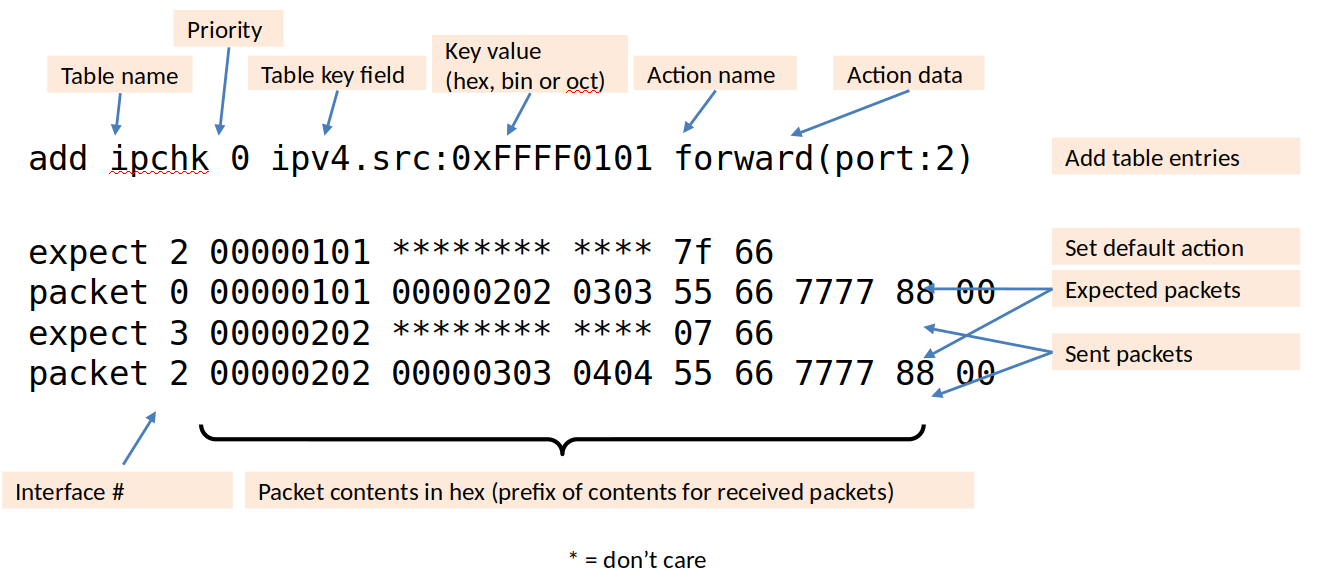
\includegraphics[width=0.7\linewidth]{stf}
	\caption{}
	\label{fig:stf}
\end{figure}
The simple test framework is a data plane verification language, which is used 
by the p4c-ebpf compiler. While its original purpose is to assess switching and 
forwarding behavior, it can also test the functionality of eBPF programs in 
isolation.
In general, an .stf file describes the input as well the expected output 
packets per switch, or in this case virtual bridge, port. In addition, it may 
also define the initial state of the dataplane tables and may contain a list of 
control plane commands which are to be run in sequence....

Compiler comes with a Python parser for STF

\subsection{The Test Runtime}
Describe the userspace runtime.
User-space wrappers around eBPF tables and APIs
\begin{figure}
	\centering
	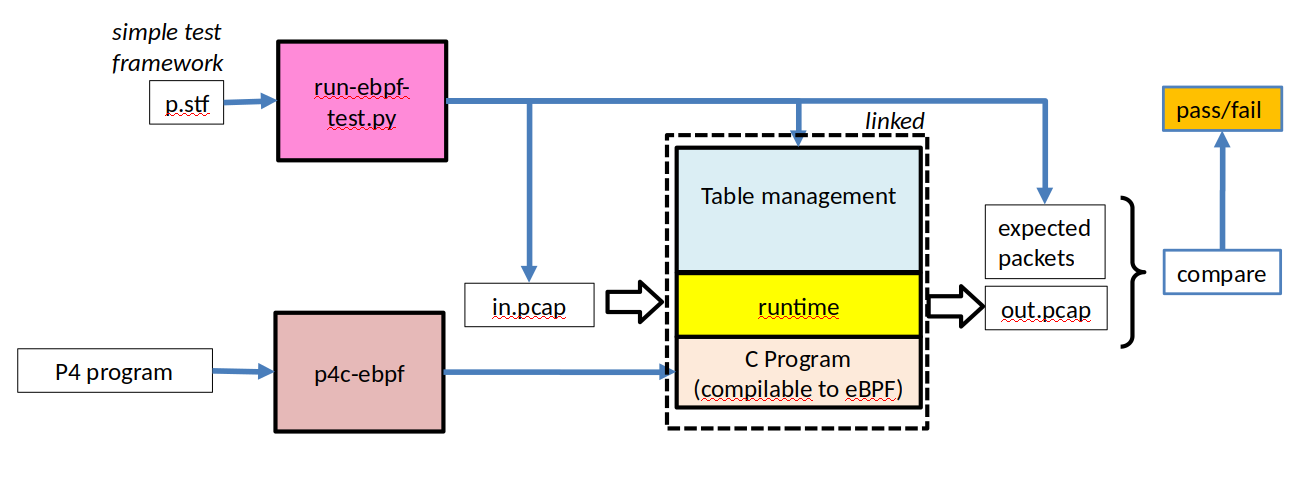
\includegraphics[width=0.7\linewidth]{user_test}
	\caption{}
	\label{fig:user_test}
\end{figure}

\subsection{Testing P4 Programs End-to-End}
Talk about how to use the test framework to verify your eBPF code or p4 file 
end-to-end. Highlight, how the framework can be used to test eBPF and XDP 
programs in general, independent from the P4 pipeline.
\begin{figure}
	\centering
	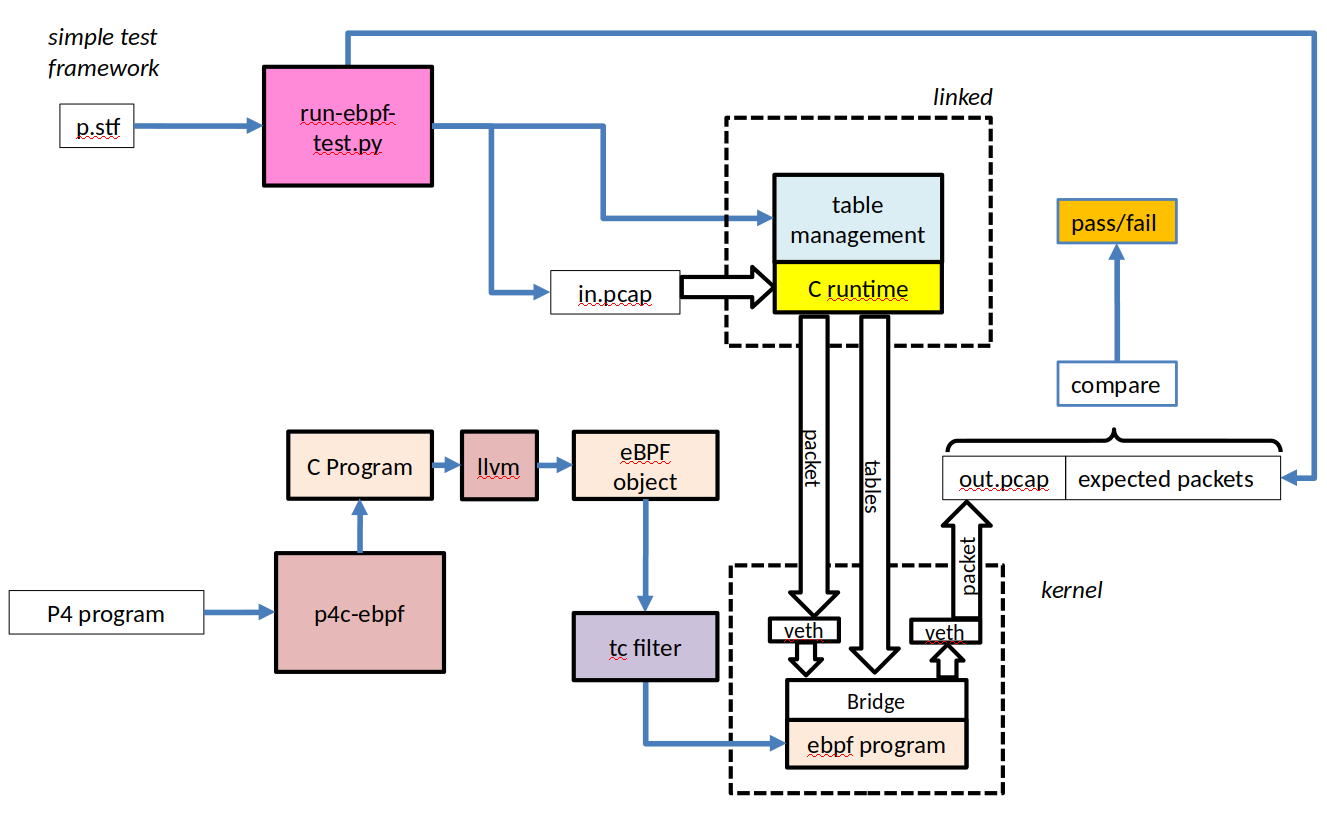
\includegraphics[width=0.7\linewidth]{kernel_test}
	\caption{}
	\label{fig:kernel_test}
\end{figure}
\section{Experimental results}\label{sec:results}
\subsection{Testbed}
All of our performance results use a hardware testbed that consists of
two Intel Xeon E5 2440 v2 1.9GHz servers, each with an Intel 10GbE X540-AT2 dual
port NIC, with the two ports of the Intel NIC on one server connected
to the two ports on the identical NIC on the other server.i
We installed p4c-xdp on one server, the {\em target server}, and
attached the XDP program to the port that receives the packets
The other server, the {\em source server}, generates packets
at the maximum 10~Gbps packet rate of 14.88~Mpps using the DPDK-based
TRex~\cite{trex} traffic generator.  The source server sends minimum
length 64-byte packets in {\em single} UDP flow to one port of the
target server, and receives the forwarded packets on the same port.
At the target server, every packet received goes through the
pipeline specified in P4.

We use sample p4 programs under the tests directory and the following
metrics to understand the performance impact of the P4-generated XDP
program:
\begin{itemize}
\item Packet Processing Rate (Mpps): Once XDP program finishes processing
the packet, it returns one of the actions mentioned in section~\ref{background}.
We made a small modification to all p4 program to always return XDP\_DROP,
so that we can count the number of packets being drop per second as a
indication of how fast the XDP can process.
\item CPU Utilization: Every packets processed by XDP program is run
under the per-core software IRQ daemon, named ksoftirqd/<core id>.
We measure the CPU utilization of the ksoftirqd on the core.
\item Number of BPF instructions verified: For each program, we list
the its max complexity; the total number of BPF instructions the
verifier has to go through, as an indication of how complicated the
program is.
\end{itemize}

The target server is running Linux kernel 4.19-rc5 and for all our
tests, the BPF JIT (Just-In-Time) compiler is enabled and JIT harden
is disabled. All programs are compiled with clang 3.8 with llvm 5.0.
For For each test program, we use the following
command from iproute2 tool to load it into kernel:
%\begin{verbatim}
\texttt{ip link set dev eth0 xdp obj xdp1.o verb}.
%\end{verbatim}

The Intel 10GbE X540 NIC is running ixgbe driver with 16 RX queues
set-up. Since the source server is sending single UDP flow, packets
always arrive at a single ring ID.  As a result, we collect the number
of packets being dropped at this ring.

\subsection{Results}
To compare the performance, we first started by manually writing two
XDP programs. The first one, SimpleDrop, does nothing but drop all packets by
returning XDP\_DROP. The second program also does nothing but returns
XDP\_TX, which forwards the packet to the receiving port.  Both programs
consists of only two BPF instructions.

{\small
\begin{verbatim}
    /* SimpleDrop */
    0: (b7) r0 = 1 // XDP_DROP
    1: (95) exit

    /* SimpleTX */
    0: (b7) r0 = 3 // XDP_TX
    1: (95) exit
\end{verbatim}
}
Then We attached the following P4 programs to the device receiving the
rate of 14.88~Mpps to evaluate the overhead introduce by the P4C-XDP
compiler.
\begin{itemize}
\item xdp1.p4: Parse Ethernet/IPv4 header, deparse it, and drop.
\item xdp3.p4: Parse Ethernet/IPv4 header, lookup an mac address
table, deparse it, and drop.
\item xdp6.p4: Parse Ethernet/IPv4 header, lookup and get a new TTL value
from eBPF map, set to IPv4 header, deparse it, and drop.
\item xdp7.p4: Parse Ethernet/IPv4/UDP header, write a pre-defined source port
and source IP, recalculate checksum, deparse, and drop.
\item xdp11.p4: Parse Ethernet/IPv4 header, swap src/dst mac address,
deparse it, and send back to the same port (XDP\_TX).
\item xdp15.p4: Parse Ethernet header, insert a customized 8-byte header,
deparse it, and send back to the same port (XDP\_TX).
\end{itemize}

\begin{table}
\centering
\small
\begin{tabular}{llll}
  \underline{P4 program} & \underline{CPU Util.} & \underline{Mpps} & \underline{Insns./Stack}\\
  SimpleDROP & 75\% & 14.4 & 2/0 \\
  SimpleTX & 100\% & 7.2 & 2/0 \\
  xdp1.p4 &  100\% &  8.1 & 277/256 \\
  xdp3.p4 &  100\% &  7.1 & 326/256 \\
  xdp6.p4 &  100\% &  2.5 & 335/272 \\
  xdp7.p4 &  100\% &  5.7 & 5821/336 \\
  xdp11.p4 &  100\% &  4.7  & 335/216 \\
  xdp15.p4 &  100\% &  5.5 & 96/56\\
\end{tabular}
\caption{\footnotesize Performance of XDP program generated by
  p4c-xdp compiler.}
\label{tab:perf}
\end{table}

As shown in Table~\ref{tab:perf}, the xdp1.p4 shows the baseline overhead
introduced by adding the parser and deparser, dropping the rate from 14.4~Mpps to
8.1~Mpps. The xdp3.p4 drops another million packet per second due to
calling the eBPF map lookup function to do a lookup, the lookup is designed
to always return NULL so no value from the map is accessed.
The xdp6.p4 shows significant overhead because it is designed to lookup
a table, find a new TTL value, and write to the IPv4 header. 
Surprisingly, the xdp7.p4 does extra parsing to the UDP header and
checksum recalculation, but the overhead is moderate due to not accessing
the table.

Finally, the xdp11.p4 and xdp15.p4 shows the transmit (XDP\_TX) performance.
Compared with xdp11 and xdp15, the xdp15.p4 involves the extra bpf\_adjust\_head helper
function to reset the pointer for extra bytes.  
Interestingly, it does not incur much over head because there is
already a reserved space in front of every XDP packet frame.

\subsection{Microbenchmark}
To further understand the performance overhead of programs generated by p4c-xdp,
we manually {\emph comments out} the entire deparser portion of the C code, so that
we can identify which stage of our XDP program (parser, lookup, and deparser) incurs
the performance overhead.

\begin{table}
\centering
\small
\begin{tabular}{llll}
  \underline{P4 program} & \underline{CPU Util.} & \underline{Mpps} & \underline{Insns./Stack}\\
  xdp1.p4 &  77\% &  14.8 & 26/0 \\
  xdp3.p4 &  100\% &  13 & 100/16 \\
  xdp6.p4 &  100\% &  12 & 98/40 \\
\end{tabular}
\caption{\footnotesize Performance of XDP program without deparser.}
\label{tab:perf2}
\end{table}

As shown in Table~\ref{tab:perf2}, the performance increases significantly.
By investigating our p4c-xdp compiler implementation and the generated C
code, we figured out that the deparser is unconditionally writing back
the entire packet content even when the P4 program does not modify any.
In addition, the deparser incurs lots of byte-order translation, e.g.,
htonl, ntohl. This could be avoided by always using network byte-order
in P4 and XDP. We leave this for future optimization.

\section{Challenges}\label{sec:conclusions}
In general, our development experience is mirrored by the lessons described 
in~\cite{minao-hspr18} and ~\cite{bertin-netdev17}.

\paragraph{No multi-/broadcast support}
While XDP is able to redirect single frames it does not have the ability to 
clone and redirect packets similar to \texttt{bpf\_clone\_redirect}. This makes 
development of more sophisticated P4 forwarding programs problematic.
\paragraph{The stack size is to small}
More complex XDP programs are rejected by the verifier despite their safeness. 
This is a particular challenge when attempting to implement network function 
chaining or more advanced pipelined packet processing in a single XDP program.

\paragraph{XDP generic and TCP}
Our testing framework uses virtual Linux interfaces and XDP \texttt{generic} 
to verify XDP programs. 
Unfortunately, we are unable to test TCP streams as the protocol is not 
supported by this driver.
Any program loaded by XDP \texttt{generic} operates after the creation of 
the \texttt{skb} and requires the original packet data. Since TCP clones every 
packet and passes the unmodifiable \texttt{skb} clone,  XDP \texttt{generic} is 
bypassed and never receives the datagram.
\paragraph{Missing userspace library}
Creating of compilation of eBPF programs in userspace requires substantial 
effort. Many function calls and variables available in sample programs are not 
available as C library and have to copied from kernel code or assembled from 
various online sources.

\paragraph{Persistent eBPF maps in namespaces}
[need to verify] When using eBPF programs in namespaces, maps exported via tc 
do not persist across \texttt{ip netns exec} calls. The consequence is that any 
program has to be run in a single shell command, otherwise the eBPF map becomes 
unusable despite the continued existence of the namespace.

\end{document}
